\documentclass[10pt]{article}
\usepackage{icmlko}

\icmlmeta{IP 파운데이션 월드모델}{320}{처음 조금은 거의 공짜다}{가중을 부분으로 걸어 절충 곡선을 그렸다 --- 볼록하고 배포 가능 구간이 있는데 거기서 아무것도 문턱을 못 넘는다}

\begin{document}

\twocolumn[
\icmlheader

\begin{abstract}
노트 319가 도메인 무게를 \emph{전부} 같게 해서 아이돌 $+$0.24 · 판 $-$0.0147
을 얻고 \textbf{배포 거절}로 끝났다. 그런데 전부-같게(모두 9.09\%)와
그대로(0.15$\sim$25.5\%) 사이가 비어 있었다. $w_i \propto n_d^{\alpha-1}$ 로
훑었다. \textbf{절충 곡선이 볼록하다} --- $\alpha{=}0.9$ 에서 아이돌
$+$0.054 인데 판은 \textbf{$-$0.0008}, $\alpha{=}0.75$ 에서 $+$0.081 에
\textbf{$-$0.0027}, $\alpha{=}0.5$ 에서 $+$0.150 에 $-$0.0134.
효율(아이돌 이득 $\div$ 판 손실)이 \textbf{68 $\to$ 28 $\to$ 11} 로 떨어진다
--- \textbf{첫 걸음이 쉰 배 싸다.} 그리고 \textbf{$\alpha{=}0.9$ 와 $0.75$ 는
배포 규칙 둘을 다 통과한다}(판이 미결정 띠 안 · 나빠진 도메인이 문턱을
안 넘음 --- 제일 나쁜 것이 애니 $-$2.66 · 도서 $-$2.26 으로 문턱 2.81 아래).
\textbf{그런데 아무것도 안 번다} --- 아이돌 이득이 $t{=}1.18$($\alpha{=}0.9$) ·
$1.53$($0.75$)로 문턱을 못 넘고 판은 그대로다. \textbf{배포 가능과 배포할
값어치는 다르다}(노트 296의 \texttt{t15} 와 같은 자리). 그래서 안 바꾼다 ---
다만 \textbf{이제 손잡이가 어디까지 공짜인지 안다.}
\end{abstract}
]

\section{사이가 비어 있었다}

노트 319는 $\alpha{=}0$(전부 같게)과 $\alpha{=}1$(지금) 두 점만 봤다.
그 사이를 $w_i \propto n_d^{\alpha-1}$ 로 훑는다 --- 도메인 총 무게가
$n_d^{\alpha}$ 에 비례한다.

\begin{figure*}[t]
\centering
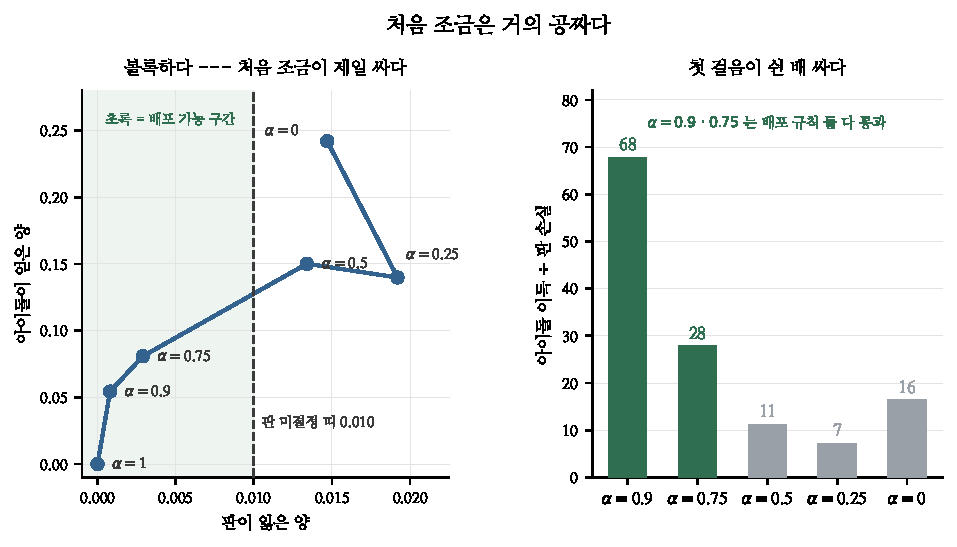
\includegraphics[width=\textwidth]{figs/convex.pdf}
\caption{왼쪽 --- 판이 잃은 양 대 아이돌이 얻은 양. 오른쪽 --- 그 비율.}
\end{figure*}

\begin{center}\small
\begin{tabular}{rrrrr}
\hline
$\alpha$ & 판 & 판 차 & 아이돌 & 도서 \\
\hline
1.00 & 0.4799 & --- & 0.1012 & 0.3895 \\
\textbf{0.90} & 0.4791 & \textbf{$-$0.0008} & \textbf{0.1555} & 0.3650 \\
\textbf{0.75} & 0.4770 & \textbf{$-$0.0029} & \textbf{0.1820} & 0.3484 \\
0.50 & 0.4665 & $-$0.0134 & 0.2513 & 0.3040 \\
0.25 & 0.4608 & $-$0.0192 & 0.2410 & 0.2736 \\
0.00 & 0.4652 & $-$0.0147 & 0.3432 & 0.2234 \\
\hline
\end{tabular}
\end{center}

\section{볼록하다}

\begin{center}\small
\begin{tabular}{rrrr}
\hline
$\alpha$ & 아이돌 이득 & 판 손실 & 효율 \\
\hline
0.90 & $+$0.054 & 0.0008 & \textbf{68} \\
0.75 & $+$0.081 & 0.0029 & \textbf{28} \\
0.50 & $+$0.150 & 0.0134 & 11 \\
0.25 & $+$0.140 & 0.0192 & 7 \\
0.00 & $+$0.242 & 0.0147 & 16 \\
\hline
\end{tabular}
\end{center}

\textbf{첫 걸음이 쉰 배 싸다.} $\alpha$ 를 1 에서 0.9 로만 내려도 아이돌이
$+$0.054 오르는데 판은 0.0008 밖에 안 잃는다 --- \textbf{판 짝SE(0.0055)의
7분의 1}이다.

\paragraph{왜 볼록한가} 노트 318의 곡선이 답이다. 아이돌 몫이 0.52\% 에서
조금만 올라도 --- 절벽 아래에서는 --- $\rho$ 가 빠르게 오른다. 반면 큰
도메인은 몫이 25\% 에서 20\% 로 줄어도 곡선의 \textbf{평평한 구간}이라 거의
안 잃는다. \textbf{한쪽은 가파른 데서 얻고 다른 쪽은 평평한 데서 잃는다.}

\section{배포 규칙은 통과하는데}

\begin{center}\footnotesize
\begin{tabular}{lrr}
\hline
& $\alpha{=}0.9$ & $\alpha{=}0.75$ \\
\hline
판 차 (① 통과) & $-$0.0007 & $-$0.0027 \\
제일 나빠진 $t$ (② 통과) & $-$2.35 & $-$2.66 \\
아이돌 & $+$0.0543 & $+$0.0808 \\
\quad $t$ (문턱 2.81) & 1.18 & 1.53 \\
진짜 몇 & 0 & 0 \\
\hline
\end{tabular}
\end{center}

\textbf{둘 다 배포 가능하다.} 판이 미결정 띠 안이고 나빠진 도메인이 문턱을
안 넘는다.

\paragraph{그런데 아무것도 안 번다} 아이돌 이득이 $t{=}1.18 \cdot 1.53$ 이라
\textbf{못 가른다.} 판은 그대로다. 진짜(문턱 넘는 도메인)가 0개다.

\begin{center}\small
\textbf{배포 가능 $\ne$ 배포할 값어치}
\end{center}

노트 296이 챔피언의 \texttt{t15} 에서 같은 자리를 봤다 --- 배포 규칙은
통과하는데 무엇을 버는지 재니 아무것도 아니었다. \textbf{규칙은 해를 거르는
장치이지 이득을 세는 장치가 아니다.}

\paragraph{그래서 안 바꾼다} $\alpha{=}1$ 을 유지한다. 바꿀 근거가 없다.
\textbf{다만 이제 손잡이가 어디까지 공짜인지 안다} --- 목표가 바뀌어
``얇은 도메인에서도 쓸 만하게''가 되면 $\alpha{=}0.75$ 가 첫 수다.

\section{곡선의 끝이 이상하다}

$\alpha{=}0.25$ 에서 판이 $-$0.0192 로 제일 나쁘고 $\alpha{=}0$ 에서 다시
$-$0.0147 로 돌아온다. 아이돌도 0.2410 $\to$ 0.3432 로 뛴다.
\textbf{단조가 아니다.}

\begin{center}\footnotesize
\begin{tabular}{ll}
\hline
가능한 까닭 & \\
\hline
잡음 & 판 짝SE 0.0055 --- 0.0045 차는 그 안이다 \\
$\alpha{=}0$ 의 특별함 & 무게가 정확히 같아지는 유일한 점 \\
\hline
\end{tabular}
\end{center}

\textbf{앞의 것이 맞을 것이다} --- 두 점 차이가 짝SE 안이다. 그래도
\textbf{곡선을 매끄럽다고 읽지 않는다}(노트 316의 규약 --- 못 가르는 값들의
순서는 못 읽는다).

\paragraph{남은 것}
\begin{center}\small
\begin{tabular}{ll}
\hline
갈래 & 왜 \\
\hline
얇은 것끼리 따로 풀 & 큰 쪽을 안 건드리는 길 \\
$\alpha$ 를 도메인마다 & 아이돌만 올리면 도서를 안 잃나 \\
\texttt{anime\_medium} & 새 축 --- 돌고 있다 \\
선형에서도 볼록한가 & F6 은 탐욕 분할이 없다 \\
\hline
\end{tabular}
\end{center}

\paragraph{규약} \textbf{두 점만 보고 절충을 판단하지 마라.} 노트 319는
$\alpha{=}0$ 과 $1$ 만 보고 ``손잡이는 옮길 뿐''로 끝냈는데, 사이를 훑으니
\textbf{효율이 68 에서 7 까지} 변한다. \textbf{절충이 선형일 이유가 없다.}
그리고 \textbf{배포 규칙을 통과했다고 배포하지 마라} --- 규칙은 해를 거르고,
이득은 따로 세야 한다. 오늘 이 판에서 그 둘을 헷갈린 자리가 두 번째다.

\end{document}
